\subsubsection{DALL-E 2} \label{sec:dall-e-2}

\textit{DALL-E 2} is a model proposed by researchers at OpenAI capable of generating images given a textual prompt~\cite{ramesh_hierarchical_2022}. This model can also modify given images, but this use case is not so interesting for the work present in this thesis.

The model consists of two blocks: the prior and the decoder. The prior converts captions into a lower-level representation, while the decoder turns this representation into an actual image.

They use \ac{CLIP} \cite{radford_learning_2021} and GLIDE (see Section~\ref{sec:glide}). For DALLE-2, the text is initially embedded using \ac{CLIP} embeddings. Then, the role of the prior is to translate these embeddings into embeddings related to an image and not the text itself. In other words, create an image representation with textual embeddings. For this, the researchers tried an \ac{AR} and a diffusion model. The diffusion one yielded better results (see Sections~\ref{sec:darn} and~\ref{sec:diffusion}). The decoder then takes the generated image representation and generates the image. The whole process can be seen in Figure \ref{fig:dall-e-2}.

\begin{figure}[ht]
    \centering
    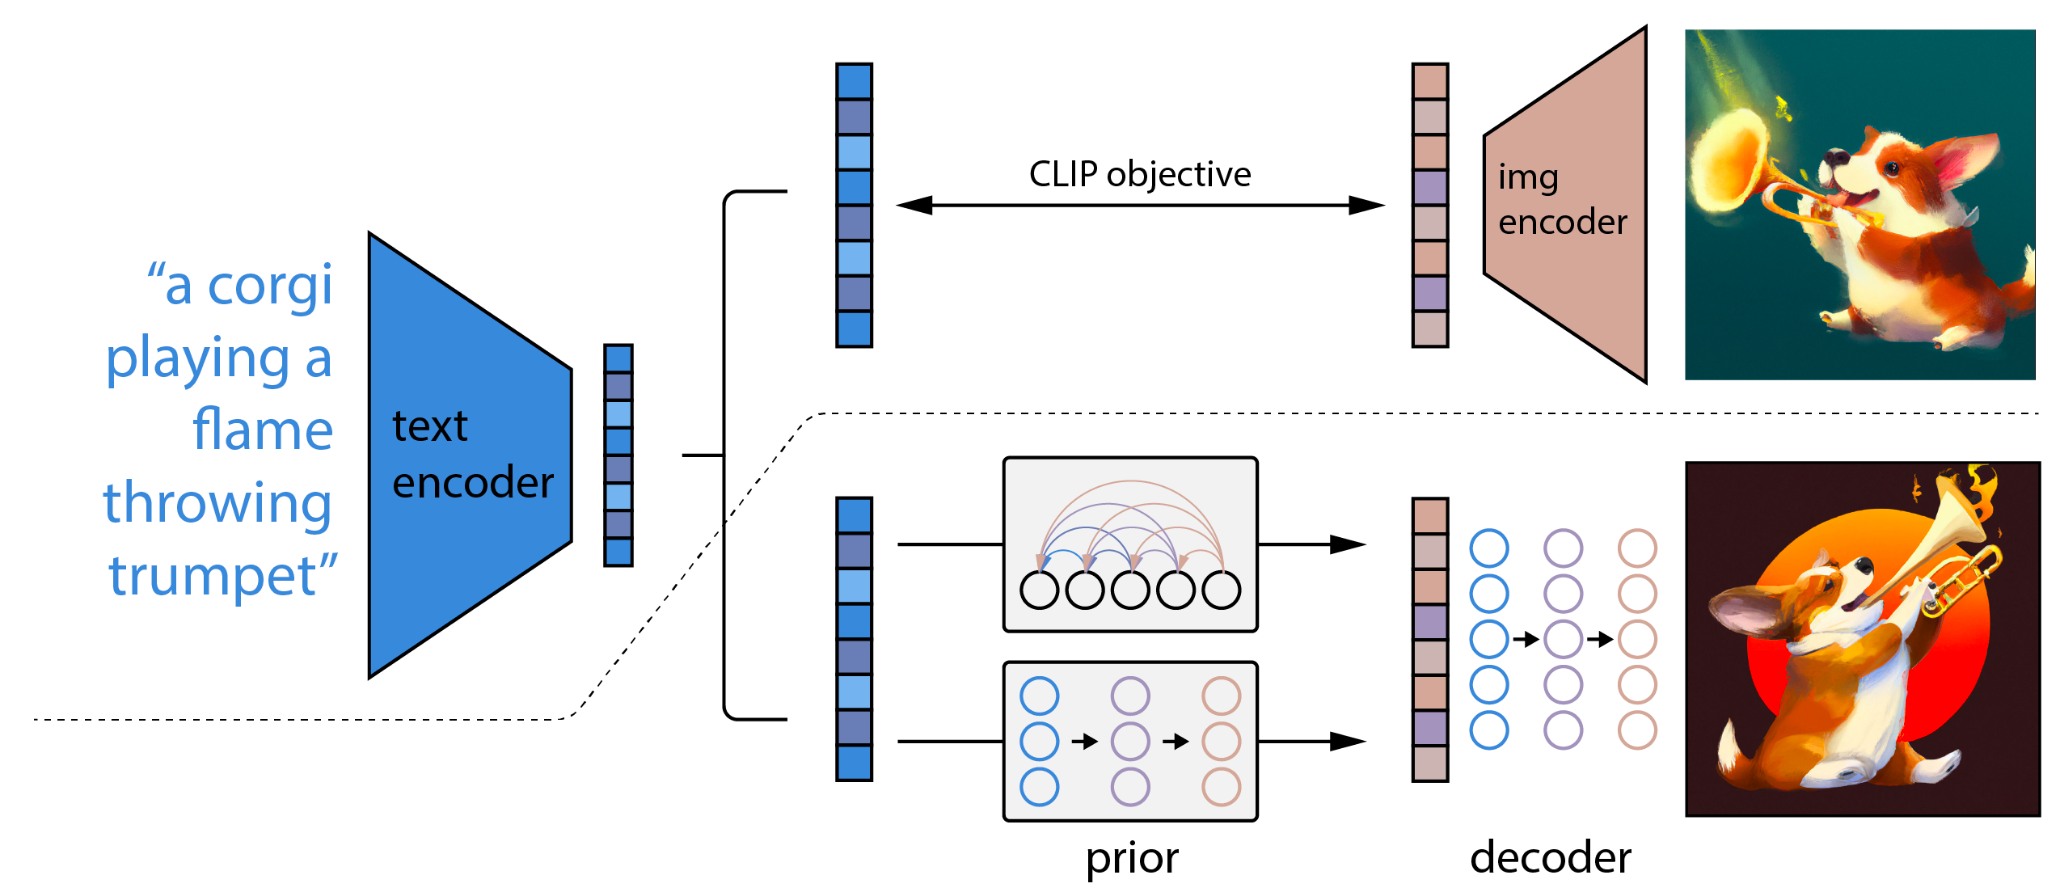
\includegraphics[width=\textwidth]{figures/2-sota/dall-e-2.png}
    \caption[DALL-E 2 architecture]{\textbf{DALL-E 2 architecture} --- The image was taken from the original paper. Above the dotted line, the \ac{CLIP} training process is depicted, where given textual and image embeddings, the \ac{CLIP} learns to translate one into the other. Below the dotted line, a text-to-image generation process is represented: a text embedding is first fed to the model that produces the image embedding. Then, this embedding is used to condition the diffusion model GLIDE which produces a final image.}
    \label{fig:dall-e-2}
\end{figure}

A model is also possible without the prior by passing the textual embeddings directly to the decoder. However, while the results were okay, they were way better with the generated image embeddings.

The decoder creates $64 \times 64$ images, but another network learns to upsample images until $1024 \times 1024$. Without this, generating high-resolution images with the decoder would make the whole operation incredibly heavy.

A significant problem of this model (and others presented here proposed by big companies) is that it needs hundreds of millions of images and an incredible amount of computation power to perform well. This highlights the importance of research toward openly accessible models such as stable diffusion (see Section~\ref{sec:stable-diffusion}).